\section{Sprachen ohne optimales Beweissystem} 
\subsection{Sprachen ohne optimales Beweissystem}

\begin{frame}
  \frametitle{Sprachen ohne optimales Beweissystem}
  
  \begin{theorem}
    Es gibt eine Sprache \(L \in \coNTIME(2^n)\), die kein optimales Beweissystem besitzt.
  \end{theorem}
\end{frame}

\subsection{Beweis}

\begin{frame}
  \frametitle{Beweisidee}

  \begin{enumerate}
   \item<1-> \(f_1, f_2, ...\): Aufzählung aller \(\FP\)-Funktionen
   \item<2-> \(L_i = 0^i10^*\) \\
              \onslide<3-> \(L_i'\) sind die Wörter aus \(L_i\), für die keine kurzen \(f_i\)-Beweise existieren \\
              \onslide<4-> \(L = \bigcup_i L_i' \in \coNTIME(2^n)\)
   \item<5-> \(L\)-Beweissystem \(f_i\): \(L_i' = L_i\), daher gibt es nur lange \(f_i\)-Beweise für \(L_i' \subset L\)
   \item<6-> Daher führt die Anname, dass \(f_i\) ein optimales Beweissystem für \(L\) ist, zum Widerspruch
  \end{enumerate}
\end{frame}

\begin{frame}
  \frametitle{Eine Aufzählung aller \(\FP\)-Funktionen}

  \begin{columns}
    \column{.7\textwidth}
      \begin{itemize}
        \item<2-> Gödel: \(M_1, M_2, ...\)
        \item<3-> \(M_1', M_2', ...\): \(M_i\) mit Wecker-Modifikation, sodass \(\runtime(M_i) \leq n^i + i\)
        \item<4-> \(f_i\): die von \(M_i\) berechnete Funktion
        \item<5-> \(n^i + i\) unbeschränkt, daher alle \(\FP\)-Funktionen
      \end{itemize}

    \column{.3\textwidth}
      \begin{figure}
        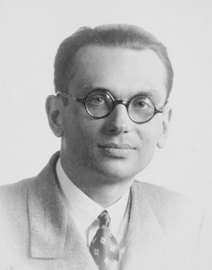
\includegraphics[width=\textwidth]{Presentation/Images/KurtGoedel.jpg}
        \caption{Kurt Gödel \\ 1906 -- 1978}
      \end{figure}
  \end{columns}
\end{frame}

\begin{frame}
  \frametitle{Konstruktion der gesuchten Sprache \(L\)}

  \begin{itemize}
    \item<1-> \(L_i = 0^i10^*\)
    \item<2-> Wähle \(x \in L_i'\), die keine kurzen \(f_i\)-Beweise haben
              \[L_i' = \{ x \in L_i : \forall_{y \in \Sigma^*} |y|^{2i} \leq 2^{|x|} \implies f_i(y) \neq x \}\]
    \item<3-> Vereinigung
              \[L = \bigcup_{i>0} L_i' \]
  \end{itemize}
\end{frame}

\begin{frame}
  \frametitle{\(L\) liegt in \(\coNTIME(2^n)\)}

  Betrachte Komplexität des Komplements
  
  \begin{itemize}
   \item<2-> \(L \in \coNTIME(2^n) \Leftrightarrow \overline{L} \in \NTIME(2^n)\)
   \item<3-> \(\overline{L} = \) \onslide<4-> \( \overline{ \bigcup_{i>0} L_i' } = \) \onslide<5-> \( \bigcap_{i>0} \overline{L_i'}\)
   \item<6-> zu zeigen: \( \bigcap_{i>0} \overline{L_i'} \in \NTIME(2^n)\)
  \end{itemize}

  \onslide<6->
  
  \(\overline{L_i'} = \{ x \in \Sigma^* : \alert<9>{ x \notin L_i } \vee \left( \alert<12>{ \exists_{y \in \Sigma^*} \left( |y|^{2i} \leq 2^{|x|} \right) } \wedge \alert<14>{ \left( f_i(y) = x \right) } \right)  \}\)

  \onslide<7-> Sei dazu \(x\) beliebiges Wort.

  \begin{itemize}
   \item<8-> Prüfe, ob \(x\) in irgendeinem \(L_i\): \onslide<9-> \alert<9>{falls nicht, dann \(x \in \overline{L}\) }
   \item<10-> Wählte \(i^*\) so, dass \(x \in L_{i^*}\)
   \item<11-> \(x \in \overline{L_j'}\) für \(j \neq i\)
   \item<12-> \alert<12>{für jedes \(y\) mit \(|y|^{2i} \leq 2^{|x|}\)}: \onslide<13-> berechne \(f_{i^*}(y)\). \onslide<14-> \alert<14>{Genau falls \(f_{i^*}(y) = x\), dann \(x \in \overline{L}\).}
  \end{itemize}

  \onslide<15>
\end{frame}


\begin{frame}
  \frametitle{Eigenschaft von Beweissystemen für \(L\)}

  Erinnerung: \(L_i' = \{ x \in L_i : \forall_{y \in \Sigma^*} |y|^{2i} \leq 2^{|x|} \implies f_i(y) \neq x \}\) \\
  und: \(\overline{L_i'} = \{ x \in \Sigma^* : x \notin L_i \vee \left( \exists_{y \in \Sigma^* \left( |y|^{2i} \leq 2^{|x|} \right) } \wedge  \left( f_i(y) = x \right) \right)  \}\)
  
  \begin{itemize}
   \item<2-> jedes Beweissystem für \(L\) ist ein \(f_i\)
   \item<3-> für dieses ist \(L_i = L_i'\)
  \end{itemize}

  \begin{itemize}
    \item<4-> sei \(f_i\) ein Beweissystem für \(L\)
    \item<5-> angenommen, es gibt ein \(x = 0^i1z \in L_i\) das nicht in \(L_i'\) liegt
    \item<6-> dann gibt es \(y\) mit \(y^{2i} \leq 2^{|x|}\) und \(f_i(y) = x\)
    \item<7-> folglich \(x \in L\) und daher \(x \in L_i'\)
  \end{itemize}
\end{frame}

\begin{frame}
  \frametitle{Widerspruch zur Existenz von optimalen Beweissystemen für \(L\)}

  Erinnerung: \(L_i' = \{ x \in L_i : \forall_{y \in \Sigma^*} |y|^{2i} \leq 2^{|x|} \implies f_i(y) \neq x \}\)

  \begin{itemize}
   \item<1-> Sei \(f_i\) optimales Beweissystem für \(L\)
   \item<2-> Sei
         \(g(bx) =
           \begin{cases}
             f_i(x) & (b=0) \\
             x      & (b = 1 \text{ and } x=0^i10^* \in L_i = L_i') 
           \end{cases}\)
   \item<3-> \(g\) ist Beweissystem für \(L\)
   \item<4-> \(f_i\) ist optimal, also ex. \(f^*\), Überführen von Beweisen: \(f_i(f^*(x)) = g(x)\), polynomiell beschränkt: \(|f^*(x)| \leq p(|x|)\)
   \item<5-> sei \(x\) aus \(L_i\), so dass \(p(|1x|)^{2i} \leq 2^{|1x|}\).
   \item<6-> \(1x\) ist \(g\)-Beweis für \(x\): \(g(1x) = x\)
   \item<7-> Dann mit \(y = f^*(1x)\): \(|y| \leq p(|1x|) \leq p(|1x|)^{2i} \leq 2^{|1x|}\).
   \item<8-> Definition von \(L_i'\): \(f_i(y) \neq x\), also \(y = f^*(1x)\) kein \(f_i\)-Beweis für \(x\)
   \item<9-> Widerspruch zur Optimalität \onslide<10-> \(\square\)
  \end{itemize}

\end{frame}

